% Created by tikzDevice version 0.6.2-92-0ad2792 on 2014-03-27 04:41:27
% !TEX encoding = UTF-8 Unicode
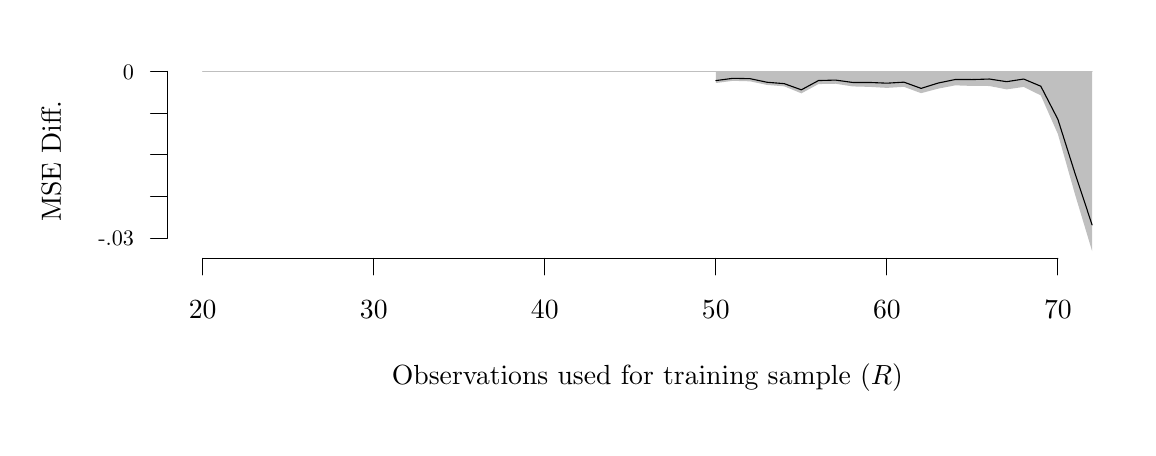
\begin{tikzpicture}[x=1pt,y=1pt]
\definecolor[named]{fillColor}{rgb}{1.00,1.00,1.00}
\path[use as bounding box,fill=fillColor,fill opacity=0.00] (0,0) rectangle (397.48,144.54);
\begin{scope}
\path[clip] ( 50.40, 61.20) rectangle (397.48,131.34);
\definecolor[named]{drawColor}{rgb}{1.00,1.00,1.00}

\path[draw=drawColor,line width= 0.3pt,line join=round,line cap=round] (248.66,124.54) --
	(254.84,125.33) --
	(261.02,125.15) --
	(267.20,123.84) --
	(273.38,123.35) --
	(279.57,120.81) --
	(285.75,124.16) --
	(291.93,124.28) --
	(298.11,123.31) --
	(304.29,123.14) --
	(310.47,122.78) --
	(316.65,123.16) --
	(322.83,120.87) --
	(329.01,122.51) --
	(335.19,123.70) --
	(341.37,123.48) --
	(347.55,123.46) --
	(353.73,122.23) --
	(359.91,123.13) --
	(366.09,120.07) --
	(372.27,106.08) --
	(378.45, 84.32) --
	(384.63, 63.80);

\path[draw=drawColor,line width= 0.3pt,line join=round,line cap=round] (248.66,125.42) --
	(254.84,126.24) --
	(261.02,126.11) --
	(267.20,124.81) --
	(273.38,124.31) --
	(279.57,122.08) --
	(285.75,125.43) --
	(291.93,125.60) --
	(298.11,124.74) --
	(304.29,124.74) --
	(310.47,124.48) --
	(316.65,124.85) --
	(322.83,122.60) --
	(329.01,124.53) --
	(335.19,125.81) --
	(341.37,125.79) --
	(347.55,125.98) --
	(353.73,125.02) --
	(359.91,125.98) --
	(366.09,123.38) --
	(372.27,111.40) --
	(378.45, 91.89) --
	(384.63, 73.27);

\path[draw=drawColor,line width= 0.3pt,line join=round,line cap=round] ( 63.25,128.74) --
	( 69.44,128.74) --
	( 75.62,128.74) --
	( 81.80,128.74) --
	( 87.98,128.74) --
	( 94.16,128.74) --
	(100.34,128.74) --
	(106.52,128.74) --
	(112.70,128.74) --
	(118.88,128.74) --
	(125.06,128.74) --
	(131.24,128.74) --
	(137.42,128.74) --
	(143.60,128.74) --
	(149.78,128.74) --
	(155.96,128.74) --
	(162.14,128.74) --
	(168.32,128.74) --
	(174.50,128.74) --
	(180.68,128.74) --
	(186.86,128.74) --
	(193.04,128.74) --
	(199.22,128.74) --
	(205.40,128.74) --
	(211.58,128.74) --
	(217.76,128.74) --
	(223.94,128.74) --
	(230.12,128.74) --
	(236.30,128.74) --
	(242.48,128.74) --
	(248.66,128.74) --
	(254.84,128.74) --
	(261.02,128.74) --
	(267.20,128.74) --
	(273.38,128.74) --
	(279.57,128.74) --
	(285.75,128.74) --
	(291.93,128.74) --
	(298.11,128.74) --
	(304.29,128.74) --
	(310.47,128.74) --
	(316.65,128.74) --
	(322.83,128.74) --
	(329.01,128.74) --
	(335.19,128.74) --
	(341.37,128.74) --
	(347.55,128.74) --
	(353.73,128.74) --
	(359.91,128.74) --
	(366.09,128.74) --
	(372.27,128.74) --
	(378.45,128.74) --
	(384.63,128.74);
\end{scope}
\begin{scope}
\path[clip] (  0.00,  0.00) rectangle (397.48,144.54);
\definecolor[named]{drawColor}{rgb}{0.00,0.00,0.00}

\node[text=drawColor,anchor=base,inner sep=0pt, outer sep=0pt, scale=  1.00] at (223.94, 15.60) {Observations used for training sample ($R$)};

\node[text=drawColor,rotate= 90.00,anchor=base,inner sep=0pt, outer sep=0pt, scale=  1.00] at ( 12.00, 96.27) {MSE Diff.};
\end{scope}
\begin{scope}
\path[clip] (  0.00,  0.00) rectangle (397.48,144.54);
\definecolor[named]{drawColor}{rgb}{0.00,0.00,0.00}

\path[draw=drawColor,line width= 0.4pt,line join=round,line cap=round] ( 63.25, 61.20) -- (372.27, 61.20);

\path[draw=drawColor,line width= 0.4pt,line join=round,line cap=round] ( 63.25, 61.20) -- ( 63.25, 55.20);

\path[draw=drawColor,line width= 0.4pt,line join=round,line cap=round] (125.06, 61.20) -- (125.06, 55.20);

\path[draw=drawColor,line width= 0.4pt,line join=round,line cap=round] (186.86, 61.20) -- (186.86, 55.20);

\path[draw=drawColor,line width= 0.4pt,line join=round,line cap=round] (248.66, 61.20) -- (248.66, 55.20);

\path[draw=drawColor,line width= 0.4pt,line join=round,line cap=round] (310.47, 61.20) -- (310.47, 55.20);

\path[draw=drawColor,line width= 0.4pt,line join=round,line cap=round] (372.27, 61.20) -- (372.27, 55.20);

\node[text=drawColor,anchor=base,inner sep=0pt, outer sep=0pt, scale=  1.00] at ( 63.25, 39.60) {20};

\node[text=drawColor,anchor=base,inner sep=0pt, outer sep=0pt, scale=  1.00] at (125.06, 39.60) {30};

\node[text=drawColor,anchor=base,inner sep=0pt, outer sep=0pt, scale=  1.00] at (186.86, 39.60) {40};

\node[text=drawColor,anchor=base,inner sep=0pt, outer sep=0pt, scale=  1.00] at (248.66, 39.60) {50};

\node[text=drawColor,anchor=base,inner sep=0pt, outer sep=0pt, scale=  1.00] at (310.47, 39.60) {60};

\node[text=drawColor,anchor=base,inner sep=0pt, outer sep=0pt, scale=  1.00] at (372.27, 39.60) {70};
\end{scope}
\begin{scope}
\path[clip] ( 50.40, 61.20) rectangle (397.48,131.34);
\definecolor[named]{fillColor}{rgb}{0.75,0.75,0.75}

\path[fill=fillColor] (248.66,128.74) --
	(248.66,124.54) --
	(254.84,125.33) --
	(261.02,125.15) --
	(267.20,123.84) --
	(273.38,123.35) --
	(279.57,120.81) --
	(285.75,124.16) --
	(291.93,124.28) --
	(298.11,123.31) --
	(304.29,123.14) --
	(310.47,122.78) --
	(316.65,123.16) --
	(322.83,120.87) --
	(329.01,122.51) --
	(335.19,123.70) --
	(341.37,123.48) --
	(347.55,123.46) --
	(353.73,122.23) --
	(359.91,123.13) --
	(366.09,120.07) --
	(372.27,106.08) --
	(378.45, 84.32) --
	(384.63, 63.80) --
	(384.63,128.74) --
	cycle;
\definecolor[named]{drawColor}{rgb}{0.75,0.75,0.75}

\path[draw=drawColor,line width= 0.4pt,line join=round,line cap=round] ( 63.25,128.74) --
	(384.63,128.74);
\definecolor[named]{drawColor}{rgb}{0.00,0.00,0.00}

\path[draw=drawColor,line width= 0.4pt,line join=round,line cap=round] (248.66,125.42) --
	(254.84,126.24) --
	(261.02,126.11) --
	(267.20,124.81) --
	(273.38,124.31) --
	(279.57,122.08) --
	(285.75,125.43) --
	(291.93,125.60) --
	(298.11,124.74) --
	(304.29,124.74) --
	(310.47,124.48) --
	(316.65,124.85) --
	(322.83,122.60) --
	(329.01,124.53) --
	(335.19,125.81) --
	(341.37,125.79) --
	(347.55,125.98) --
	(353.73,125.02) --
	(359.91,125.98) --
	(366.09,123.38) --
	(372.27,111.40) --
	(378.45, 91.89) --
	(384.63, 73.27);
\end{scope}
\begin{scope}
\path[clip] (  0.00,  0.00) rectangle (397.48,144.54);
\definecolor[named]{drawColor}{rgb}{0.00,0.00,0.00}

\path[draw=drawColor,line width= 0.4pt,line join=round,line cap=round] ( 50.40, 68.44) -- ( 50.40,128.74);

\path[draw=drawColor,line width= 0.4pt,line join=round,line cap=round] ( 50.40, 68.44) -- ( 44.40, 68.44);

\path[draw=drawColor,line width= 0.4pt,line join=round,line cap=round] ( 50.40, 83.51) -- ( 44.40, 83.51);

\path[draw=drawColor,line width= 0.4pt,line join=round,line cap=round] ( 50.40, 98.59) -- ( 44.40, 98.59);

\path[draw=drawColor,line width= 0.4pt,line join=round,line cap=round] ( 50.40,113.67) -- ( 44.40,113.67);

\path[draw=drawColor,line width= 0.4pt,line join=round,line cap=round] ( 50.40,128.74) -- ( 44.40,128.74);

\node[text=drawColor,anchor=base east,inner sep=0pt, outer sep=0pt, scale=  0.80] at ( 38.40, 65.68) {-.03};

\node[text=drawColor,anchor=base east,inner sep=0pt, outer sep=0pt, scale=  0.80] at ( 38.40,125.99) {0};
\end{scope}
\end{tikzpicture}
